\documentclass{beamer}
\usepackage{pgfpages}
\usepackage[backend=bibtex]{biblatex}
\usepackage{multicol}
\usepackage{multimedia}
\usepackage[absolute,overlay]{textpos}
\usepackage{parskip}
\usepackage{hyperref}
\usepackage{lmodern}
\usepackage{caption}
\hypersetup{colorlinks=true, urlcolor=blue}
\setlength{\parskip}{\smallskipamount} 
%\usepackage[texcoord,grid,gridunit=mm,gridcolor=red!10,subgridcolor=green!10]{eso-pic} %DELETE when done with grid
\setbeameroption{hide notes} % Only slides
%\setbeameroption{show only notes} % Only notes
%\setbeameroption{show notes on second screen=right} % Both
%\bibliography{../../papers/references.bib}
\setbeamerfont{footnote}{size=\tiny}
%\AtEveryCitekey{\clearfield{title}}

%
% Choose how your presentation looks.
%
% For more themes, color themes and font themes, see:
% http://deic.uab.es/~iblanes/beamer_gallery/index_by_theme.html
%
\mode<presentation>
{
  \usetheme{Warsaw}      % or try Darmstadt, Madrid, Warsaw, ...
  \usecolortheme{default} % or try albatross, beaver, crane, ...
  \usefonttheme{default}  % or try serif, structurebold, ...
  \setbeamertemplate{navigation symbols}{}
  \setbeamertemplate{caption}[numbered]
} 

\usepackage[english]{babel}
%\usepackage[utf8x]{inputenc} %Doesn't play well with biblatex
\usepackage{amssymb}
\usepackage{bm}
\usepackage{color}
\usepackage{graphicx}

\newcommand{\red}[1]{{\color{red}{#1}}}

\title[{\color{white}{Day 3}}]{{\Huge TIP and Color Blindness} \\ {\normalsize Clubes de Ciencia - Ensenada 2017 \\ Frank Wilzcek Course}}
\author{Cody Petrie \& David Rojas}
\institute{Universidad Aut\'onoma de Baja California}
\date{}
\titlegraphic{
\includegraphics[width=2cm]{../../logos/CdeC_logo.png}~%\hspace*{0.75cm}~
   
\includegraphics[width=1.5cm]{../../logos/UABC_logo.png}
}

\begin{document}

%\setbeamertemplate{frametitle}[default][center]
\begin{frame}
   \titlepage
\end{frame}

% Uncomment these lines for an automatically generated outline.
%\begin{frame}{Outline}
%  \tableofcontents
%\end{frame}

% Commands to include a figure:
%\begin{figure}
%\includegraphics[width=\textwidth]{your-figure's-file-name}
%\caption{\label{fig:your-figure}Caption goes here.}
%\end{figure}

\begin{frame}{Digital Representation of Images}
   \begin{itemize}
      \item The standard digital representation of colored images is simple, conceptually.
      \item The pixels form a 2-dimensional matrix, whose entries are the coordinates in some (normally) 3-dimensional color space, RGB.
      \item It's important to realize that the R, G, B used in practical work are not spectral red, green and blue - far from it (as you will measure).
   \end{itemize}
\end{frame}

\begin{frame}{Digital Representation of Images}
\begin{figure}[ht]
   \begin{minipage}[b]{0.45\linewidth}
      \centering
      
\includegraphics[width=\textwidth]{figures/data.jpg}
      \\ 500x380 pixels
   \end{minipage}
   \hspace{0.5cm}
   \begin{minipage}[b]{0.45\linewidth}
      \centering
      
\includegraphics[width=\textwidth]{figures/data_crop.pdf}
      \\ 15x15 pixels
   \end{minipage}
\end{figure}
~\\ Each pixel contains 3 numbers, so the 15x15 picture has 15x15x3=675 numbers.
\end{frame}

\begin{frame}{Manipulating Images}
   \begin{center}
      \Huge \textcolor{blue}{Manipulating Images}
   \end{center}
\end{frame}

\begin{frame}{Manipulating Images}
   \begin{itemize}
      \item Since the information about an image is stored digitally, as numbers, it is easy to manipulate.
      \item To do image processing, one does mathematical operations on the numbers, thus generating a new processed image data file, and then translates that file back into a processed image.
   \end{itemize}
   \begin{center}
      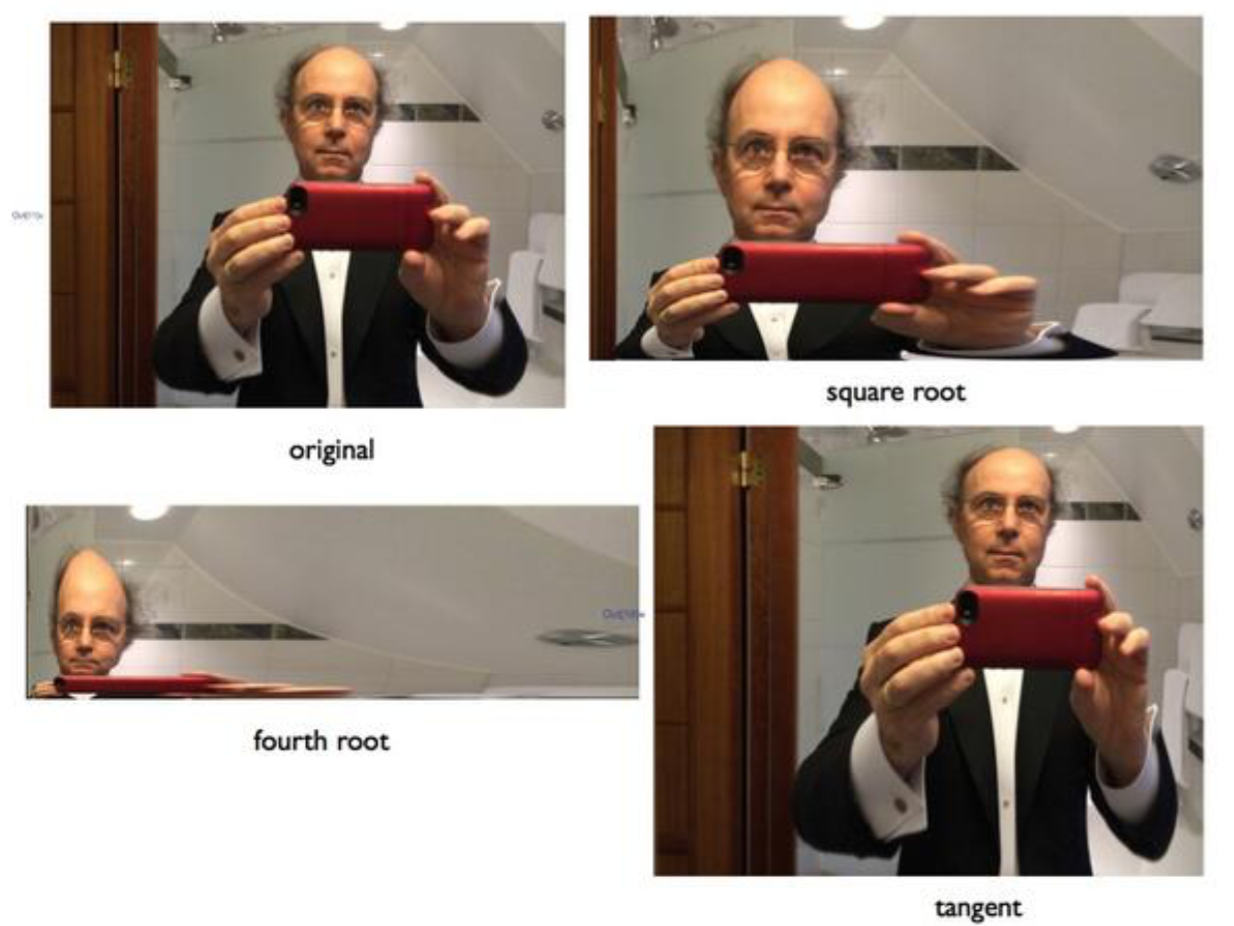
\includegraphics[width=0.7\textwidth]{figures/frank.png}
   \end{center}
\end{frame}

\begin{frame}{Manipulating Images}
   \begin{itemize}
      \item Python supports a rich toolkit for image manipulation, as does (for example) Mathematica.
      \item You have been working in the Python ecosystem. You might also enjoy playing with Mathematica and browsing in its excellent documentation.
      \item Highly recommended for background and context:
      \begin{itemize}
         \item \href{http://reference.wolfram.com/language/guide/ ImageProcessing.html}{http://reference.wolfram.com/language/guide/ ImageProcessing.html}
         \item This goes into many important topics we will not cover, notably feature detection.
      \end{itemize}
   \end{itemize}
\end{frame}

\begin{frame}{Hyperspectral Information}
   \begin{center}
      \Huge \textcolor{blue}{The Challenge of Hyperspectral Information}
   \end{center}
\end{frame}

\begin{frame}{Hyperspectral Information}
   \begin{itemize}
      \item As we've seen in our color-tone work, it can be fun to bring out more than three information channels in images (while retaining the spatial structure).
      \item The tone strategy is effective locally, but it is ill- suited to giving a global picture.
      \item It would be powerful to do something similar to all the pixels at once, in a visual display but our visual color system projects to only three dimensions, however many we try to force-feed it.
      \item Problem: How can we get past that limitation?
   \end{itemize}
\end{frame}

\begin{frame}{Curing Red-Green color blindness}
   \begin{itemize}
      \item Before discussing TIP in a general way, it will be good to look at an instructive example: We will use it to ``cure" color blindness.
      \item Let's look at Red-Green color blindness for example.
   \end{itemize}
   \begin{center}
      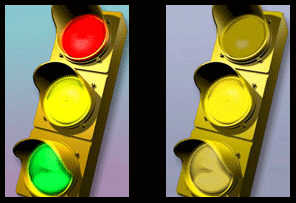
\includegraphics[width=0.7\textwidth]{figures/stoplight.jpg}
   \end{center}
\end{frame}

\begin{frame}{Curing Red-Green color blindness}
   \begin{itemize}
      \item A crude but roughly correct way to simulate the most common form of color blindness - red-green color blindness - is to replace the {R, G, B} content of each pixel in an image by { (R+G)/2, (R+G)/2, B}. Let’s call this operation RGA (for red green averaging).
      \item Images that appear the same to a trichromat after RGA will appear the same to a dichromat even before RGA.
      \item Images that appear different to a trichromat after RGA will also appear different to a dichromat after RGA.
      \item The RGA projection allows trichromats to visualize the difficulty dichromats encounter in the standard Nishihara test for color blindness:
   \end{itemize}
\end{frame}

\begin{frame}{Curing Red-Green color blindness}
What number do you see?
~\\~
\begin{figure}[ht]
   \begin{minipage}[b]{0.45\linewidth}
      \centering
      \uncover<2->{
      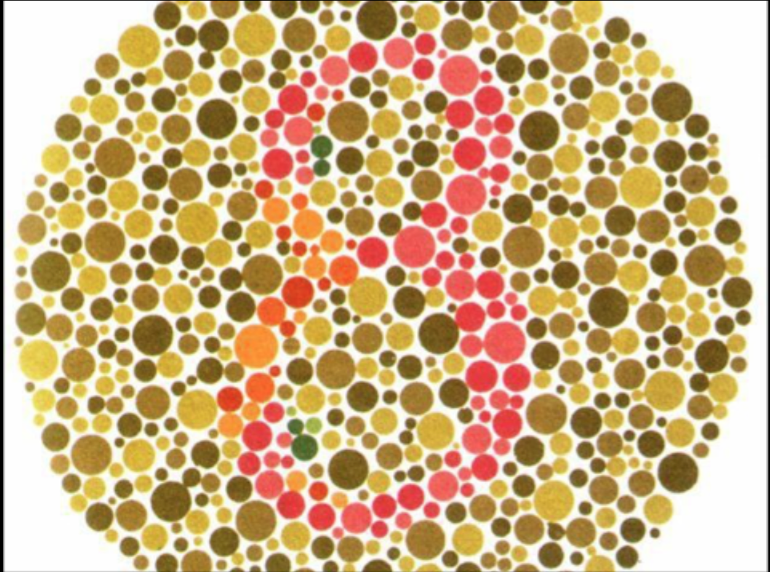
\includegraphics[width=\textwidth]{figures/RGAbefore.png}
      }
      \\ Before RGA
   \end{minipage}
   \hspace{0.5cm}
   \begin{minipage}[b]{0.45\linewidth}
      \centering
      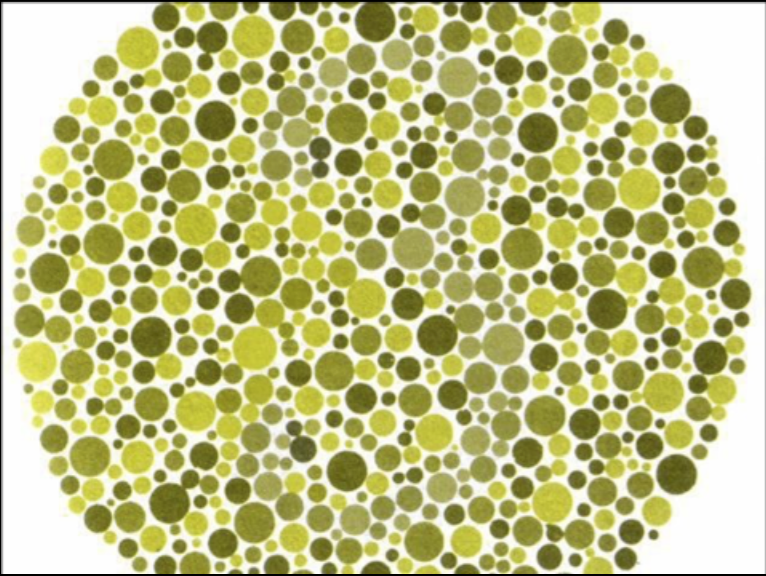
\includegraphics[width=\textwidth]{figures/RGAafter.png}
      \\ After RGA
   \end{minipage}
\end{figure}
\uncover<2>{
The RGA projection allows trichromats to visualize the difficulty dichromats encounter in the standard Nishihara test for color blindness.
}
\end{frame}

\begin{frame}{Exploiting the Time Dimension(s)}
   \begin{itemize}
      \item By encoding the missing information as a time- dependent modulation of the signal which is unaffected by RGA, we can make it available to dichromats.
      \item This can be done in many ways. Some simple, reasonably effective ones involve formulas like this:
      \begin{equation*}
         {R,G,B} \rightarrow {Rf(t) + Gg(t), Rf(t)+Gg(t),B}
      \end{equation*}
      \item where $f$ and $g$ are two different functions of time. (Note that R = G as displayed.)
   \end{itemize}
\end{frame}

\begin{frame}{Exploiting the Time Dimension(s)}
   \begin{center}
      Here is what you get with $f(t)=\cos^2kt$, $g(t)=\sin^2kt$: \\~\\
      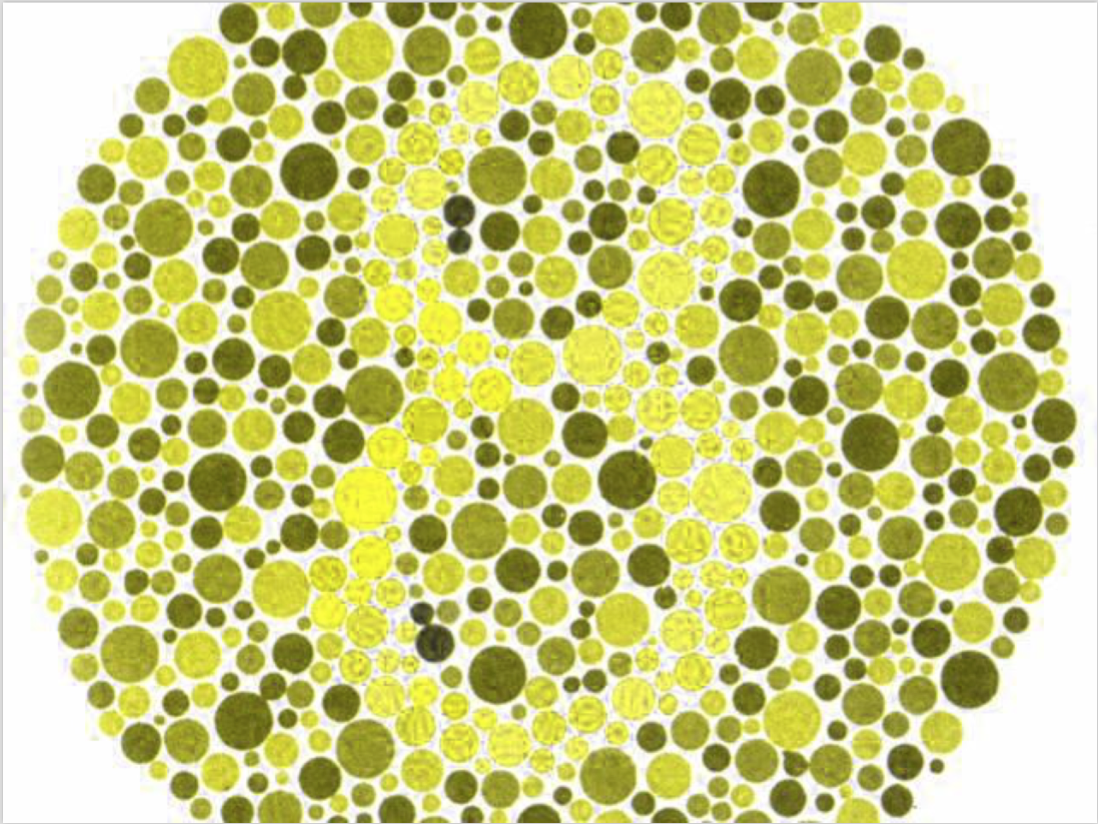
\includegraphics[width=0.6\textwidth]{figures/timefix.png}
      \\~\\
   \end{center}
\end{frame}

\begin{frame}{Exploiting the Time Dimension(s)}
   \begin{center}
      And here is what you get with an encoding where $f$ and $g$ have slightly probabilistic features:
      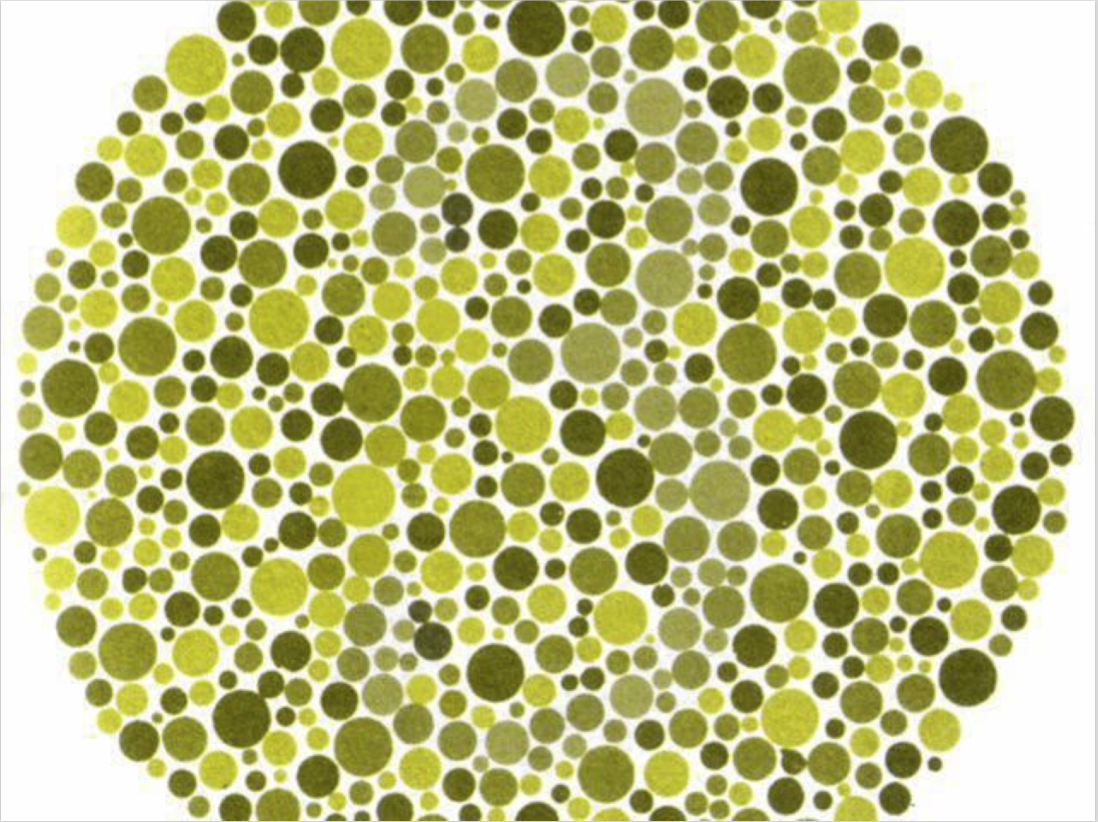
\includegraphics[width=0.6\textwidth]{figures/probfix.png}
      \\ In a larger sense, we are all nearly color-blind.
   \end{center}
\end{frame}

\begin{frame}{Exploiting the Time Dimension(s)}
   This becomes strikingly evident if you plot differential sensitivities of the opsins as a function of spectral wavelength:
   \begin{center}
      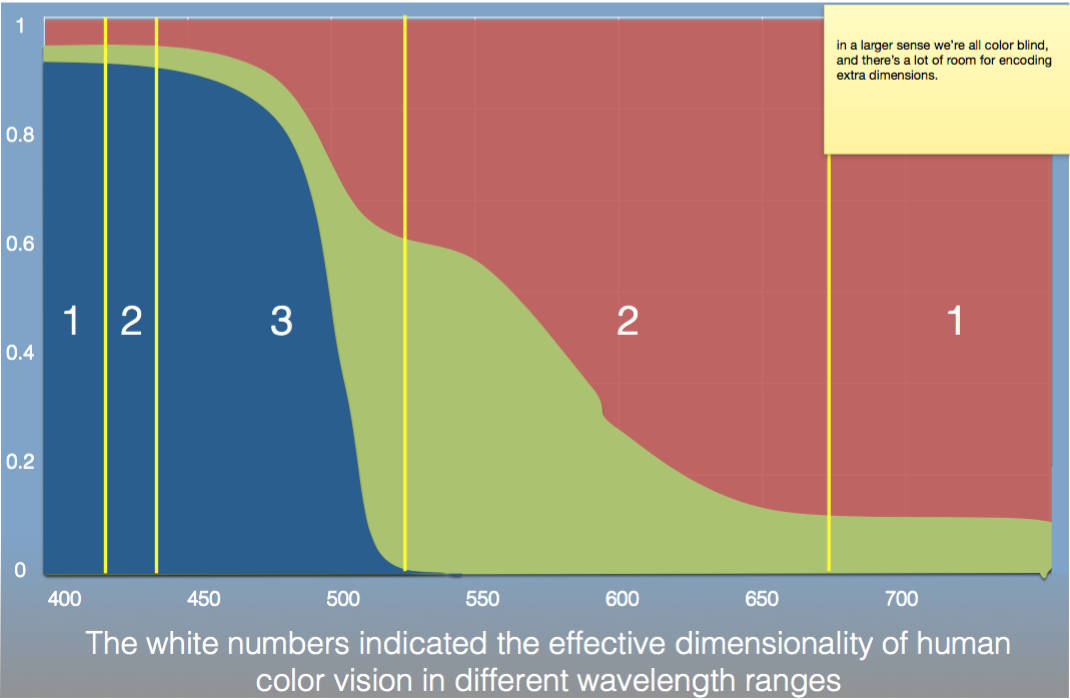
\includegraphics[width=0.9\textwidth]{figures/spectralsensativity.png}
   \end{center}
\end{frame}

\begin{frame}{Exploiting the Time Dimension(s)}
   \begin{itemize}
      \item But we can use TIP to open up extra channels.
      \item Previously, we used TIP to go from a 2-dimensional color space (after RGA) to a 3-dimensional color space. But essentially the same trick will allow us to go from 3 to 4, or more.
      \item To be concrete, let's imagine we want to resolve Green into Olive and Cyan:
   \end{itemize}
\end{frame}

\begin{frame}{Exploiting the Time Dimension(s)}
   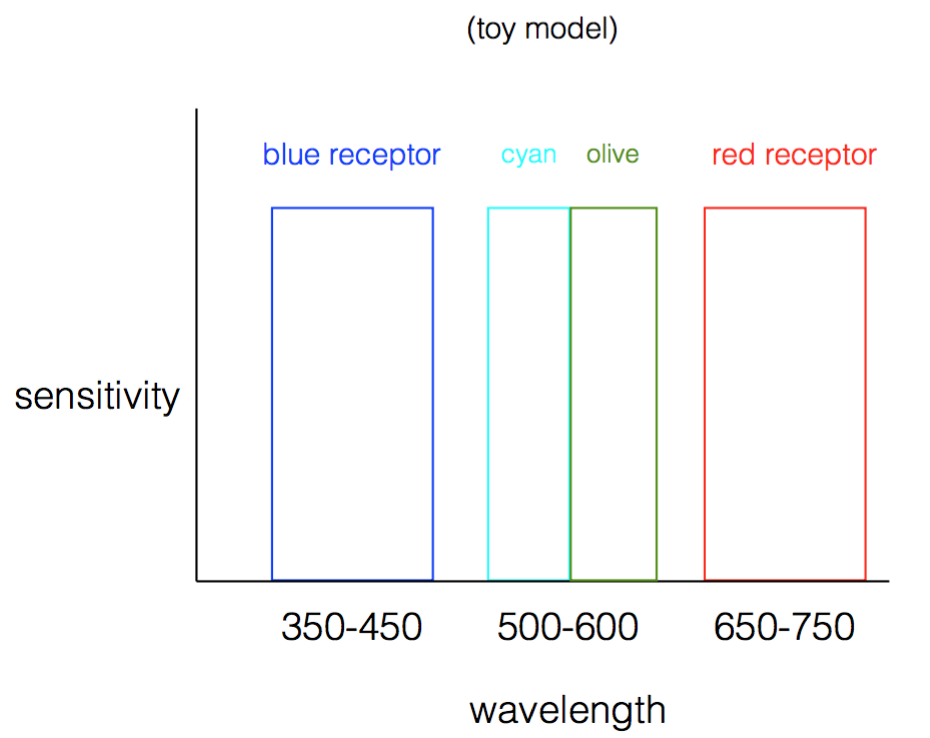
\includegraphics[width=0.9\textwidth]{figures/cyanolive.png}
\end{frame}

\begin{frame}{Exploiting the Time Dimension(s)}
   \begin{itemize}
      \item Again, there are many ways to do this. In our toy model, perhaps the most natural is to put all the action in the G channel:
      \begin{equation}
         {R,G,B} \rightarrow {R, Of(t)+Cg(t),B}
      \end{equation}
      \item It is an open question, what are the most effective and attractive TIP methods to transmit hyperspectral, and more generally extra-dimensional, information.
      \item You'll get to explore this issue.
   \end{itemize}
\end{frame}

\begin{frame}{Varieties of Color Vision}
   \begin{center}
      \Huge \textcolor{blue}{Varieties of Color Vision in the Animal World}
   \end{center}
\end{frame}

\begin{frame}{Varieties of Color Vision}
   \begin{center}
      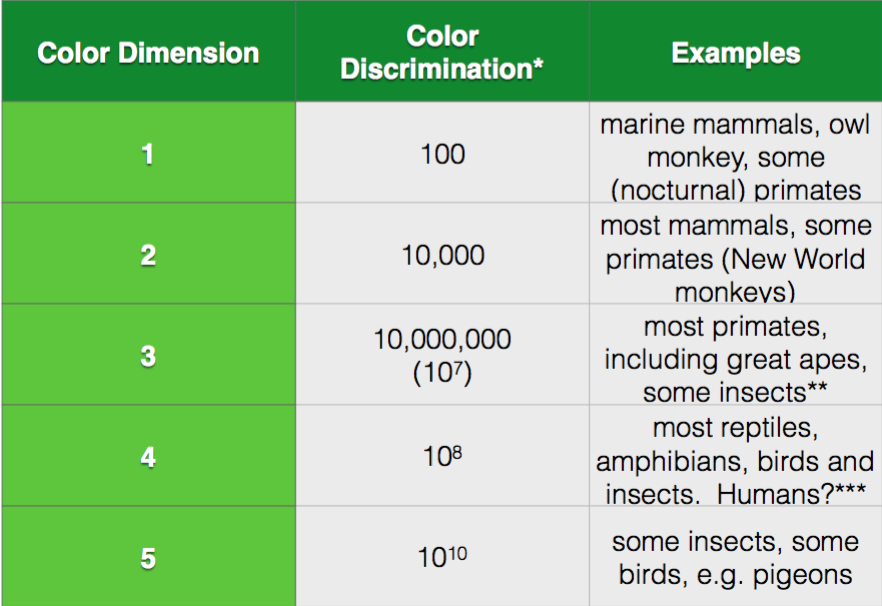
\includegraphics[width=0.9\textwidth]{figures/colordiscrimination.png}
      \\ *These numbers are rough estimates, and not to be trusted.
   \end{center}
\end{frame}

\begin{frame}{Varieties of Color Vision}
Mantis Shrimp seems to be the champ:
   \begin{center}
      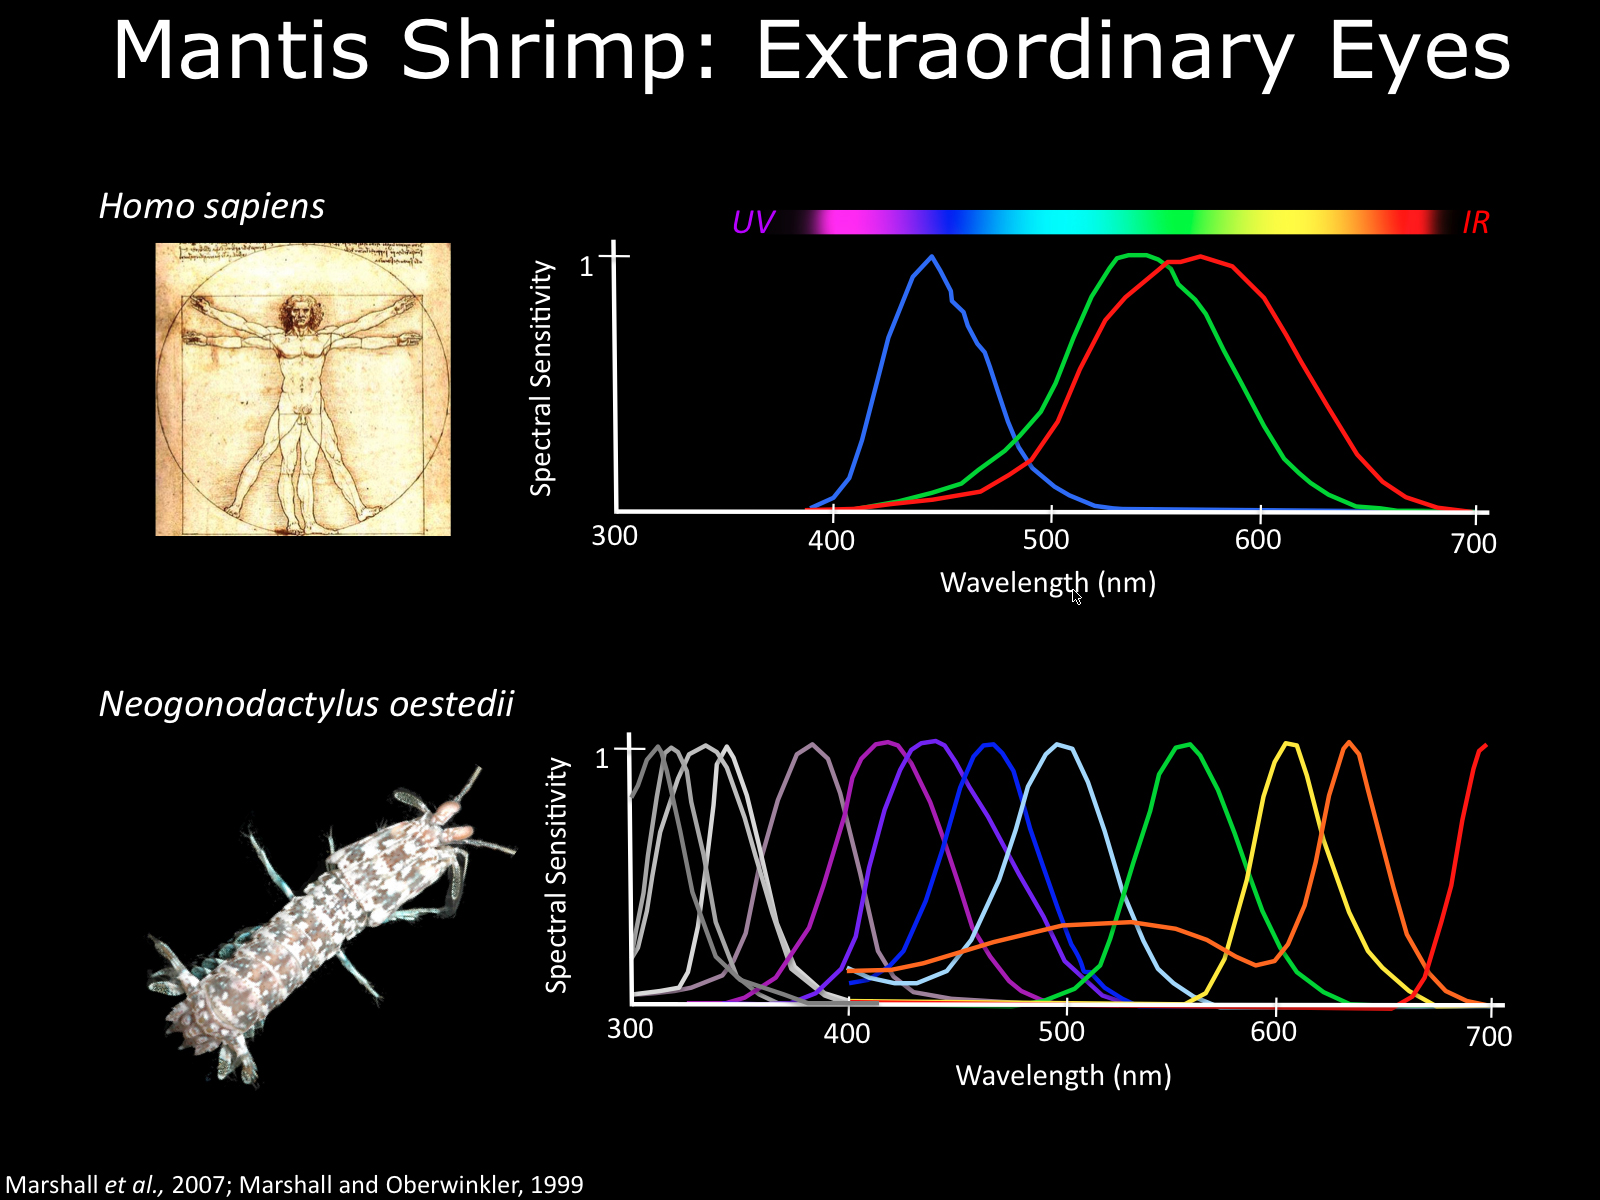
\includegraphics[width=0.9\textwidth]{figures/mantisshrimp.jpg}
   \end{center}
\end{frame}

\begin{frame}{Varieties of Color Vision}
   \begin{itemize}
      \item Most non-primate mammals are less capable (in different ways):
   \end{itemize}
   \begin{center}
      
\includegraphics[width=0.6\textwidth]{figures/redroses.jpg}
   \end{center}
\end{frame}

\begin{frame}{Varieties of Color Vision}
   \begin{center}
      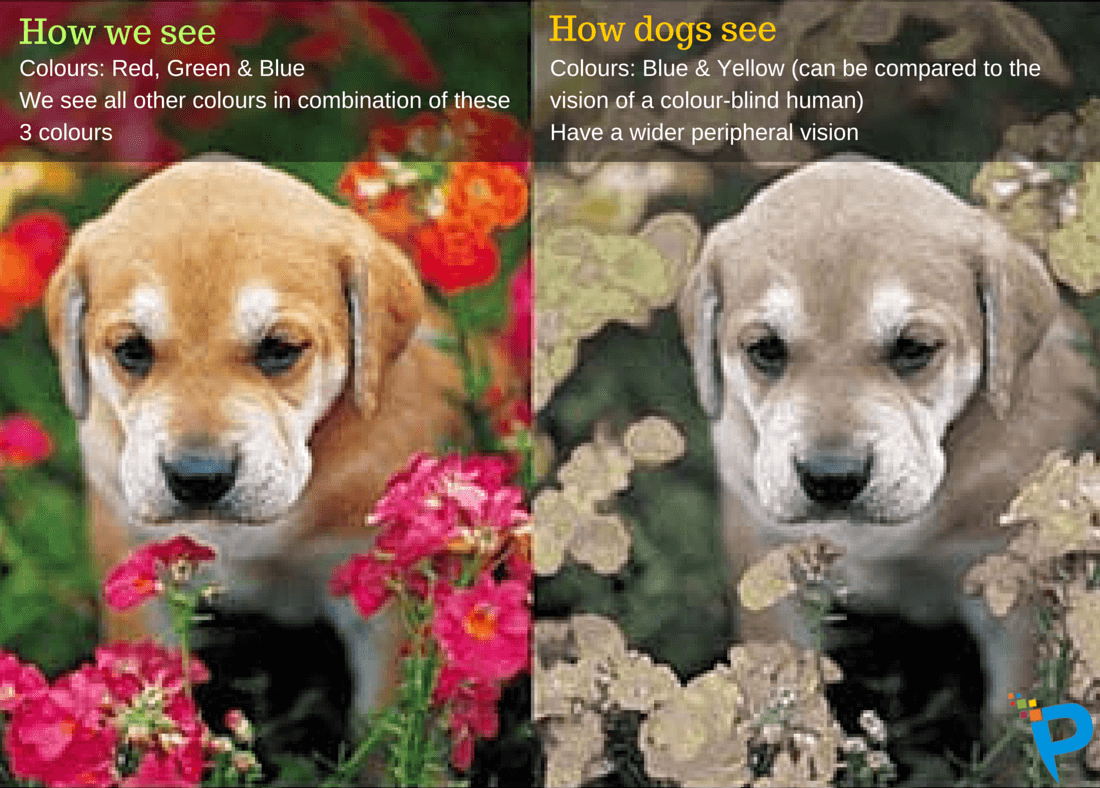
\includegraphics[width=0.9\textwidth]{figures/dogvison.png}
      \\ We can mimic these variations in software or hardware.
   \end{center}
\end{frame}

\begin{frame}{Varieties of Color Vision}
   \begin{center}
      It's interesting and relevant to note that insect and crustacean eyes are based on radically different principles from our ``imaging" eyes. \\
      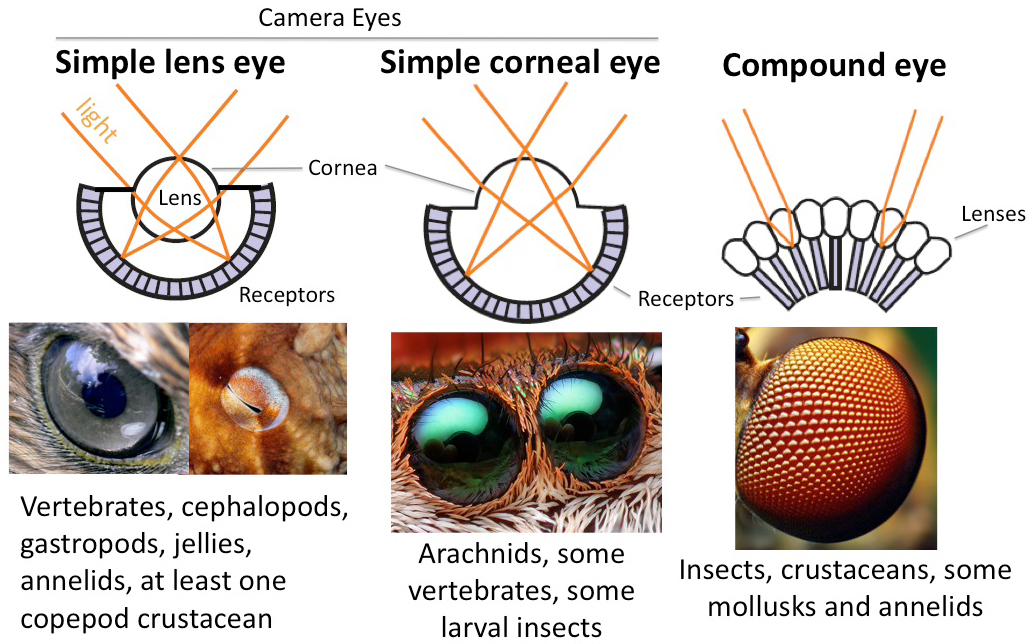
\includegraphics[width=0.9\textwidth]{figures/insecteyes.jpg}
   \end{center}
\end{frame}

\begin{frame}{Varieties of Color Vision}
   \begin{itemize}
      \item There's some evidence that a small percentage of women exhibit tetrachromacy. Thus they can discriminate colors that elude most humans.
   \begin{center}
      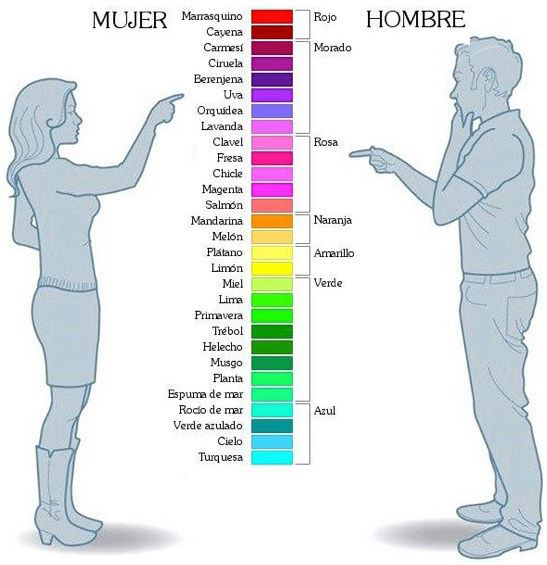
\includegraphics[width=0.6\textwidth]{figures/womenvsmencolors.jpg}
   \end{center}
   \end{itemize}
\end{frame}

\begin{frame}{Dichromats and Tetrachromats}
   \begin{center}
      \Huge \textcolor{blue}{More About Dichromats and Tetrachromats}
   \end{center}
\end{frame}

\begin{frame}{Dichromats and Tetrachromats}
   \begin{itemize}
      \item The most common type of color blindness is ``deuteroanomaly", which affects about 6\% of males.
      \item Deuteroanomalous individuals still have three kinds of opsins and cone cells, but their ``green" opsin contains a mutation, which shifts its sensitivity curve toward red.
      \item Thus they have two closely similar receptors, which gives less resolving power.
   \end{itemize}
   \begin{center}
      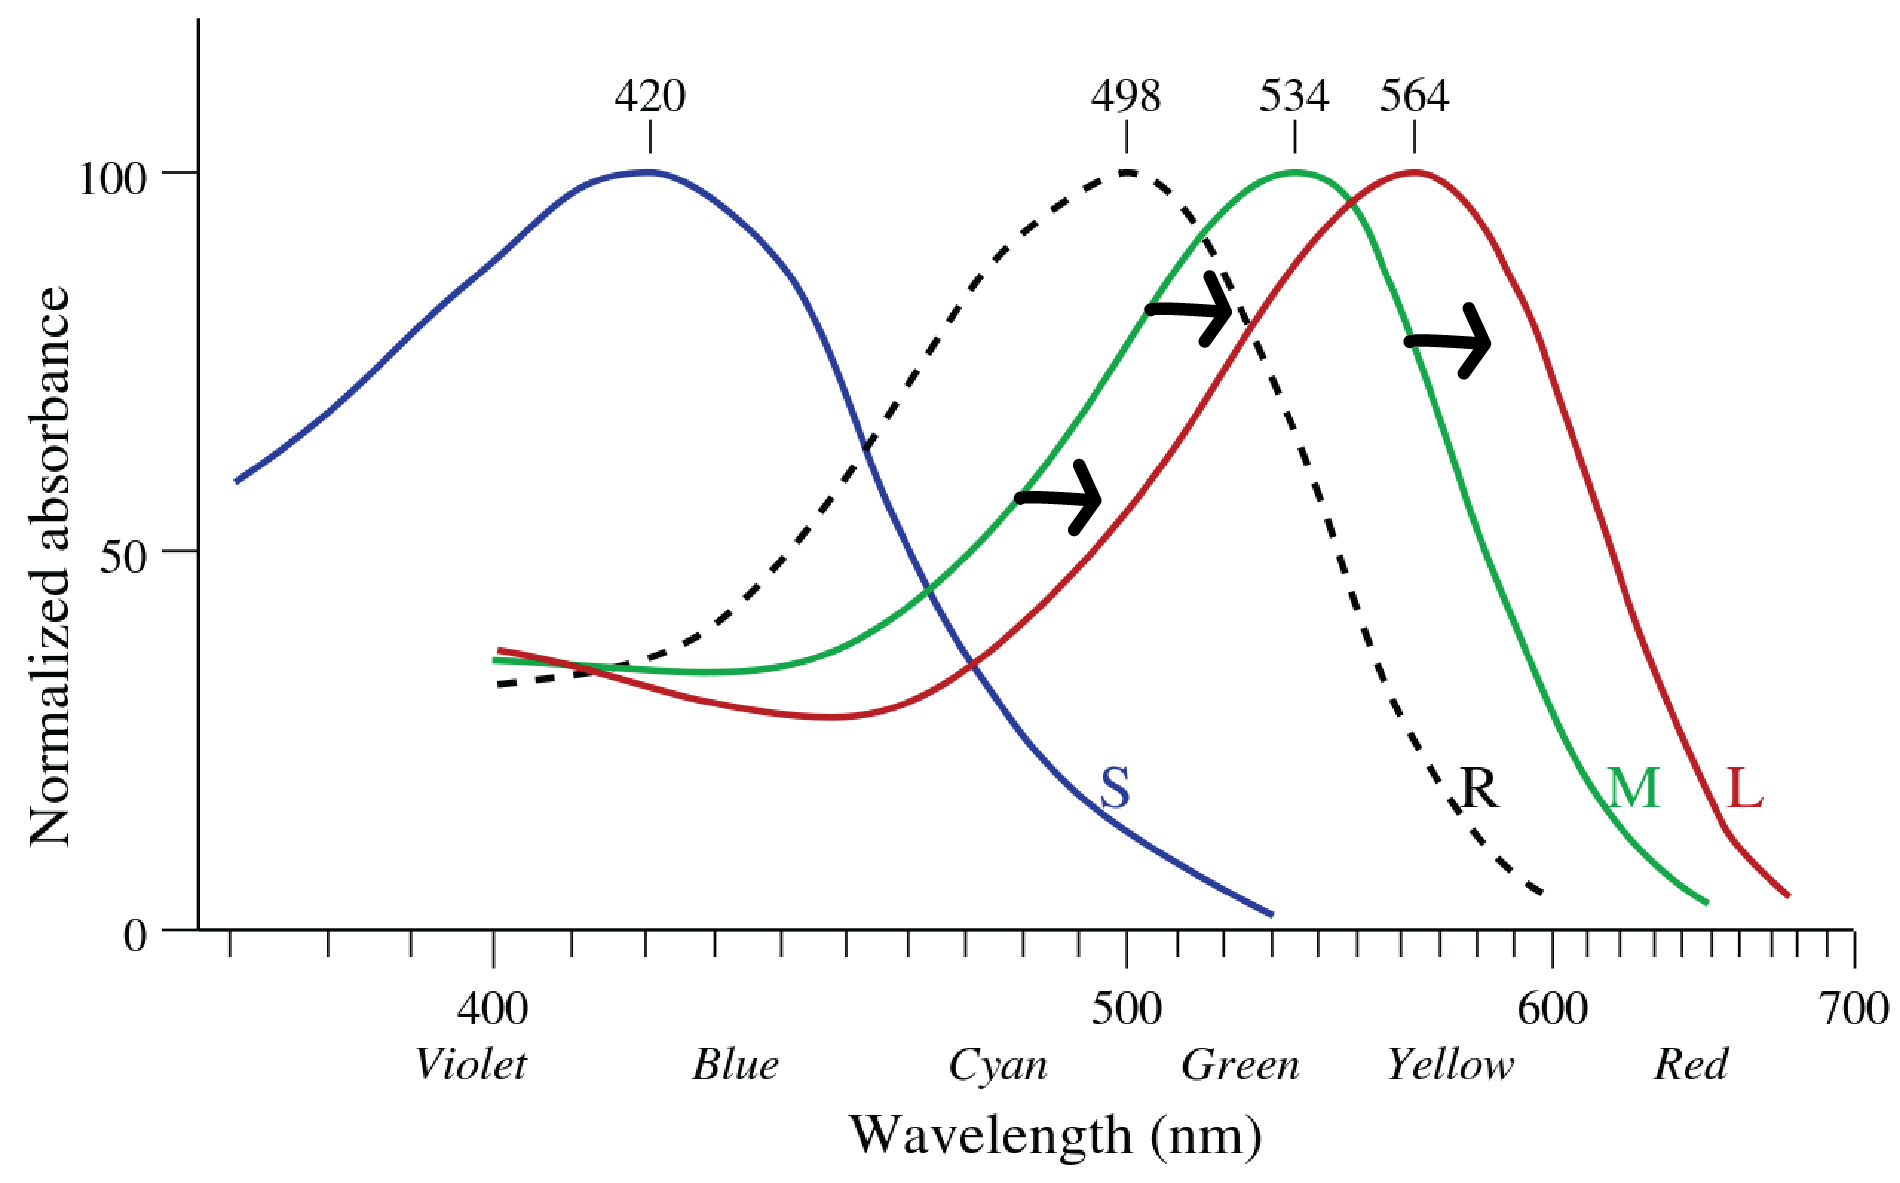
\includegraphics[width=0.7\textwidth]{figures/deuteroanomaly.png}
   \end{center}
\end{frame}

\begin{frame}{Dichromats and Tetrachromats}
A simple example
   \begin{center}
      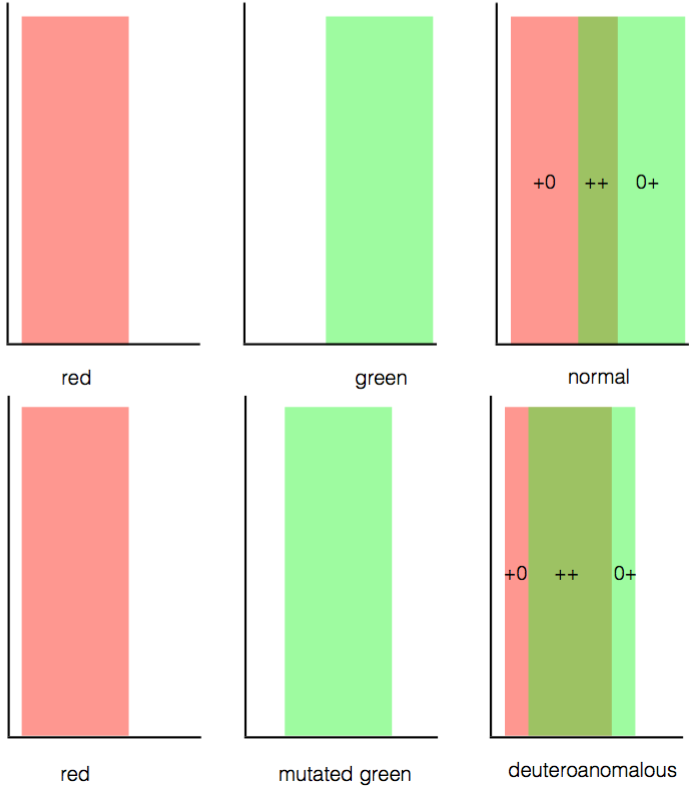
\includegraphics[width=0.6\textwidth]{figures/redgreenbars.png}
   \end{center}
\end{frame}

\begin{frame}{Dichromats and Tetrachromats}
   \begin{columns}
   \begin{column}{0.15\textwidth}
      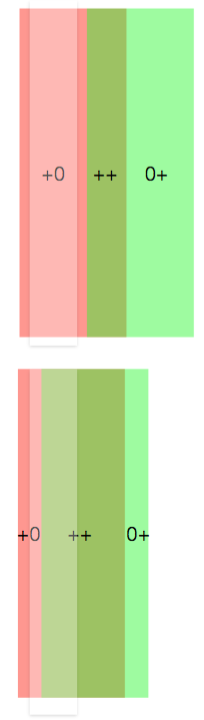
\includegraphics[width=1.4\textwidth]{figures/redgreenbars2.png}
   \end{column}
   \begin{column}{0.85\textwidth}
      \begin{itemize}
         \item On comparing these diagrams, several disadvantages of our model ``deuteroanomalous" opsins are evident. There is a larger ++ zone, wherein frequencies are not discriminated, narrower opposition zones, and a significant new blind region.
         \\~\\
         \item On the other hand, if the illumination is heavily weighted toward red, the deuteroanomalous opsins are {\it advantaged}.
      \end{itemize}
   \end{column}
   \end{columns}
\end{frame}

\begin{frame}{Dichromats and Tetrachromats}
   \begin{itemize}
      \item One simple yet striking conclusion is clear and robust: Deuteroanomalous ``color blind" individuals actually can resolve some (red-heavy) color combinations that look the same to normal trichromats.
      \item It would be a nice project to demonstrate this directly.
      \item You'll be making tools which are adequate to that task.
   \end{itemize}
\end{frame}

\begin{frame}{Dichromats and Tetrachromats}
   \begin{itemize}
      \item The mutated green opsin gene is carried on the X chromosome.
      \item Thus males, (one X chromosome), are susceptible to red-green deuteroanomalous (RGD) color blindness.
   \end{itemize}
   \begin{center}
      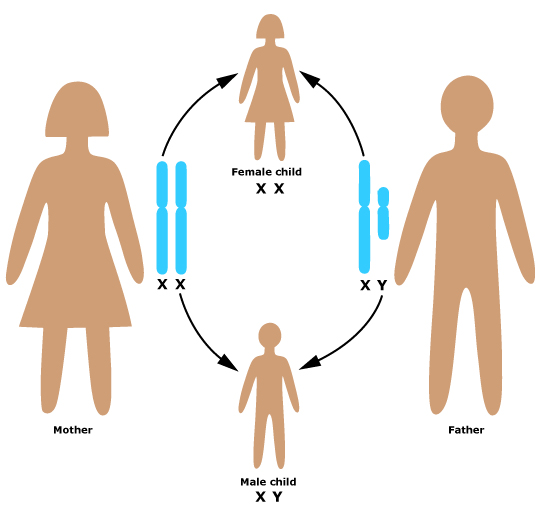
\includegraphics[width=0.6\textwidth]{figures/XY.jpg}
   \end{center}
\end{frame}

\begin{frame}{Dichromats and Tetrachromats}
   \begin{itemize}
      \item On the other hand, females may carry both the normal and the mutated green opsins, one on each of their two X chromosomes.
      \item If both are expressed, in different cone cells, the individual will have four different opsins altogether, and she will be a tetrachromat.
      \item We should expect this for sisters and daughters of RGD males, and in about 9\% of females altogether.
   \begin{center}
      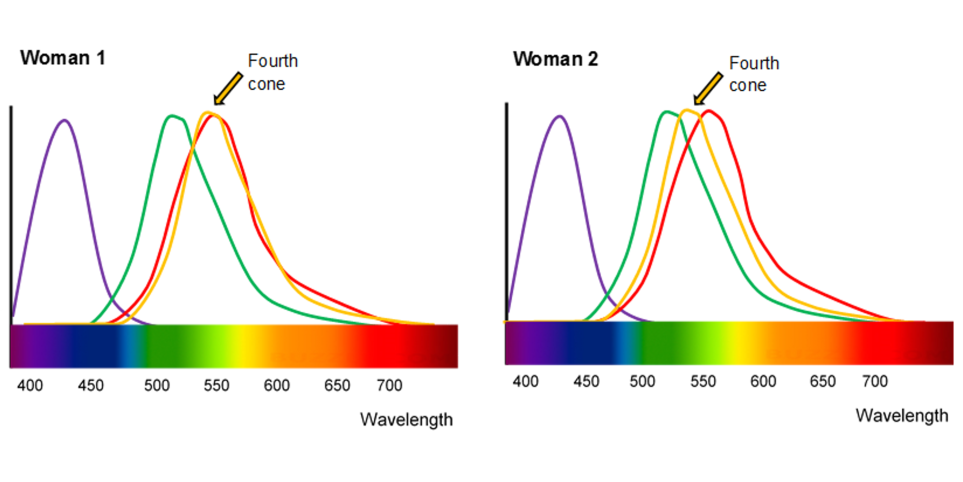
\includegraphics[width=0.85\textwidth]{figures/fourcones.png}
   \end{center}
   \end{itemize}
\end{frame}

\begin{frame}{Dichromats and Tetrachromats}
   \begin{itemize}
      \item The manifestations of this sort of tetrachromacy might be rather subtle, since two of the opsins - red and mutated green - have very similar receptive characteristics.
      \item But the same tests that bring out extra resolving power in RGD males should also bring out this sort of tetrachromacy.
   \end{itemize}
\end{frame}

\begin{frame}{Picture Citations} 
\fontsize{5}{4}\selectfont  
CdeC logo (accessed 13 July 2017): \href{https://www.clubesdeciencia.mx}{https://www.clubesdeciencia.mx}\\
UABC logo (accessed 13 July 2017): \href{http://www.uabc.mx/}{http://www.uabc.mx/}\\
Star Trek (accessed 17 July 2017): \href{https://s-media-cache-ak0.pinimg.com/736x/00/78/05/0078051e2a16b50fe5cbede33bd2a38e--star-trek-data-star-trek-jokes.jpg}{https://s-media-cache-ak0.pinimg.com/736x/00/78/05/0078051e2a16b50fe5cbede33bd2a38e--star-trek-data-star-trek-jokes.jpg}
Stop light (accessed 18 July 2017): \href{http://www.moondragon.org/health/disorders/eyecolorblindness.html}{http://www.moondragon.org/health/disorders/eyecolorblindness.html}
Mantis shrimp spectrum (accessed 14 July 2017): \href{http://greenforkutah.blogspot.com/2014/07/how-you-can-tell-if-mantis-shrimp-has.html}{http://greenforkutah.blogspot.com/2014/07/how-you-can-tell-if-mantis-shrimp-has.html}\\
Roses are gray (accessed 18 July 2017): \href{https://s-media-cache-ak0.pinimg.com/736x/58/08/38/5808384b6901685847b8e2109d5979fc--love-poems-poor-dog.jpg}{https://s-media-cache-ak0.pinimg.com/736x/58/08/38/5808384b6901685847b8e2109d5979fc--love-poems-poor-dog.jpg}\\
Dog vison (accessed 18 July 2017): \href{http://www.punditcafe.com/science/human-vs-animal-vision-cat-bee-snake-shark-dog-vision/}{http://www.punditcafe.com/science/human-vs-animal-vision-cat-bee-snake-shark-dog-vision/}\\
Women vs. men colors (accessed 18 July 2017): \href{http://www.taringa.net/posts/ciencia-educacion/15532817/Las-mujeres-ven-mas-colores-que-los-hombres.html}{http://www.taringa.net/posts/ciencia-educacion/15532817/Las-mujeres-ven-mas-colores-que-los-hombres.html}\\
Deuteroanomaly (accessed 18 July 2017): \href{https://thebrainissocool.com/2015/03/08/is-the-grass-redder-or-greener-on-the-other-side/}{https://thebrainissocool.com/2015/03/08/is-the-grass-redder-or-greener-on-the-other-side/}\\
Chromosomes (accessed 18 July 2017): \href{https://s-media-cache-ak0.pinimg.com/originals/2b/aa/77/2baa77adc3058c3e931fb49713148caf.jpg}{https://s-media-cache-ak0.pinimg.com/originals/2b/aa/77/2baa77adc3058c3e931fb49713148caf.jpg}\\
Four cones (accessed 18 July 2017): \href{https://theneurospherecom.files.wordpress.com/2015/12/candidates.png?w=963}{https://theneurospherecom.files.wordpress.com/2015/12/candidates.png?w=963}
\end{frame}

\end{document}
